%%%%%%%%%%%%%%%%%%%%%%%%%%%%%%%%%%%%%%%%%%%%%%%%%%%%%%%%%%%%%%%%%%%
%                                                                 %
%                            CHAPTER THREE                          %
%                                                                 %
%%%%%%%%%%%%%%%%%%%%%%%%%%%%%%%%%%%%%%%%%%%%%%%%%%%%%%%%%%%%%%%%%%%

\chapter{ANALYSIS} \label{sec:analysis}

After the GZGC concluded, we reprocessed and reanalyzed all images contributed by all citizen scientists.  For consistency, and to ensure accuracy, this included the images submitted for feedback generation during collection.   All images across all client machines were accumulated and given to a server for processing.  The accumulated analysis with IBEIS completed the following steps:

%The complete results of a participant's $N_i$ processed images could be made available by publicly hosting it or otherwise delivered for viewing, although this was not done for the GZGC. For a publicly-visible viewing, the identification code on the registration card would allow participants to not only locate their complete results but will also provide some level of anonymity to other participants and to the administrators of the event for blind analysis

\begin{enumerate}
    \item IBEIS semi-automatically found detection regions (i.e.\ bounding boxes around potential sightings) of zebras (and giraffes) in all of the images contributed by all citizen scientists.
    \item A reviewer manually checked the detection regions by altering poor detections, removing false-positive detections, and adding missed detections.
    \item A reviewer manually added relevant metadata to the detections, including viewpoint of the animal and the quality of the sighting for that animal.
    \item A filtering step eliminated detections that violated the collection protocol (non-left viewpoint images) or were considered of insufficient quality.
    \item IBEIS incrementally processed each surviving sighting to find matching animals from the recognition database.
    \item A reviewer used the results of the appearance-based matching and the IBEIS interface to either assign a new name to the unknown individual or mark it as a repeated sighting.
    \item A reviewer identified \textit{split} and \textit{join} name scenarios, described in Section \ref{sec:identification}, where an error occurred during the name assignment.
    \item After naming was completed, a final review step allowed a trained biologist to age and sex the individual using all of its sightings.
\end{enumerate}

For each of the review steps, a review interface was added to IBEIS to help streamline and parallelize the work of manually reviewing (i.e.\ \textit{turking}) the results.  These \textit{turking interfaces} have been fully integrated into IBEIS as a web interface and are shown in Figures \ref{fig:turking_interface_detection}, \ref{fig:turking_interface_viewpoint}, \ref{fig:turking_interface_quality}, and \ref{fig:turking_interface_metadata}.  It should be noted that the IBEIS software processed the sightings incrementally, in chronological order, such that the assigned name identifiers of newly sighted animals followed the order of when they were sighted during the GZGC.

All turking interfaces were designed with high parallelization and accuracy in mind.  Because of these attributes, the turking interfaces were implemented as a web portal that would allow a reviewer to access a series of unreviewed detection regions or to assign viewpoint, age, or sex metadata to an already reviewed detection region.  To accomplish the parallelization, the interfaces employed randomization to prevent two or more reviewers from working on the same image.  Every time the web turking web page was refreshed in the internet browser, a new, random, and unreviewed image was given to the reviewer.

It should be noted that no locking, checkout, or reservation system was employed to implement the parallelized system.  The lack of a reservation system did introduce some duplicated turking effort as the number of unreviewed images began to decease (to around twice the number of active reviewers) because two reviewers could have been given the same random image to annotate.  However, this cost was considered worth paying as it significantly reduced the complexity of the overall turking system.  In practice, this scheme worked well for our turking problem because the time it took for a reviewer to review an image was generally very short, from less than 1 second to 10 seconds.  In the event an image was randomly selected more than once (and given to two different reviewers) before being marked as reviewed, the last submitted reviewer's decision recorded over all previous reviewer's decision.  This inefficiency was the inherent trade-off paid to forgo a much more sophisticated reservation system.

As an optional feature, the turking interfaces allowed for an administrator mode that provided a verification procedure during annotation.  When an image was submitted by a reviewer, a random selection (10 percent) was mirrored to an administrator's monitor for review.  If the administrator agreed with the reviewer's decision, nothing more needed to be done and no action needed to be completed; conversely, if the administrator disagreed, the event gave the administrator and reviewer a chance to reconcile the inconsistency and administer further training to adhere with the turking protocol.  The turking system kept a running average of each reviewer's success and failure rates.  When that ratio fell below a specified threshold for a particular reviewer, that individual was suggested to take a break or undergo an additional session of training.

\begin{figure}[t]%
%\begin{figure}[!htb]%
    \centering
    \subfloat {{ $\vcenter{\hbox{ 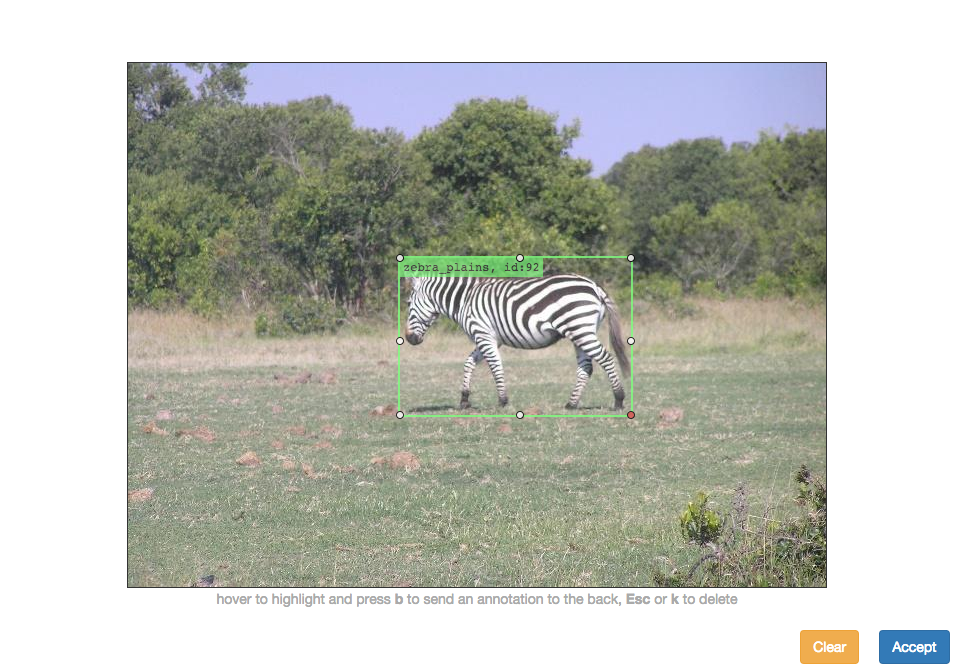
\includegraphics[width=0.75\textwidth]{resources/turk_detection.png} }}$ }}%
        \caption[The Detection Region Turking Web Interface]{\textbf{The Detection Region Turking Web Interface.}  The detection web interface allowed a reviewer to add (or remove) detection regions (bounding boxes) to an image.  The detection regions were to signify the locations of animals in the image.  All animals were annotated by the reviewer except for when an animal was too small or obscurred.  The interface also allowed for bounding box resizing, translation, and deletion.}
        \label{fig:turking_interface_detection}
\end{figure}

\section{Detection}
After the automatic image detection processing was completed by IBEIS, a reviewer had to manually check for poor detections (bounding boxes that did not properly constrain the individual), false detections that weren't actually zebras (false-positives), and missed detections of zebras (false-negatives).  The detection regions were annotated using a click-and-drag interface, which is a very common interaction design for computer interfaces and a natural motion for detection region annotation.  The detection regions had 8 control points for resizing the detection region and also allowed for moving, rotating, and deleting.  IBEIS automatically gave a species to the detection region, but this could be later corrected by a reviewer.  An example image being reviewed in the web interface for appropriate detection regions can be seen in Figure \ref{fig:turking_interface_detection}.  After the image detections were reviewed, a second review procedure was started in order to increase the accuracy of animal identification by adding quality and viewpoint information to the reviewed annotation.

For detection regions, the optimal scenario was to put a bounding box around the entire animal in the frame of the image.  However, due to occlusion from the natural landscape, occlusion from other animals, or poorly framed animals (as seen in Figure \ref{fig:qualities} (b)) sometimes the detection region could not accommodate a bounding box around the entire individual.  For these sightings, a best-fit procedure was followed: try to maximize coverage of the entire animal but prevent significant brush or other animals from being seen inside the bounding box.  The guiding principle when selecting a representative bounding box around an individual was to give the IBEIS identification system as much detail as possible about the foreground, target individual and minimize the amount of distraction from brush or other animals.  In practice, this meant that the resulting annotations fluctuated significantly in pose, viewpoint, size, coverage, and usable detail.  However, as long as identifying marks could be seen in the detection region, the identification system should have been able to find a corresponding match in the database.

\begin{figure}[t]%
%\begin{figure}[!htb]%
    \centering
    \subfloat {{ $\vcenter{\hbox{ 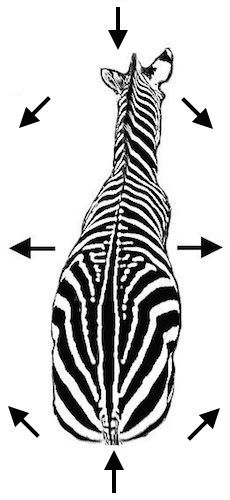
\includegraphics[width=0.25\textwidth]{resources/guideline_inverted.jpg} }}$ }}%
        \caption[The Viewpoint Orientation Bins Allowed by IBEIS]{\textbf{The Viewpoint Orientation Bins Allowed by IBEIS.}  The different orientations allowed by IBEIS (0-360) binned into the 8 cardinal and sub-cardinal viewpoints.  The reference point for annotating viewpoint was based on the location of the camera in relation to the animal.  For example, if the animal was facing towards the camera (head looking into the camera), then the correct viewpoint annotation is down; conversely, if the animal was facing away and to the right, then the correct viewpoint annotation is up and to the right.}
        \label{fig:viewpoint}
\end{figure}

\section{Viewpoint and Quality}
The need to annotate the viewpoint of the animal was required to facilitate more accurate appearance-based identification results by filtering queried images and the corresponding matches.  As mentioned in Chapter \ref{sec:collection}, plains zebras (and Masai giraffes) are not left-right symmetric.  Thus, IBEIS could only identify animals taken from a consistent viewpoint, which, for the purposes of the GZGC, was the left side.  The viewpoint annotation on the images allowed IBEIS to limit the input to the identification pipeline and to filter the returned matches from IBEIS to have agreeing viewpoints.

Viewpoint information was added to the detected animal as a discretized integer from 0-360 degrees (where 0 degrees signified a left viewpoint) and then binned into the following eight 45-degree semantic viewpoints: \textit{left} (0), \textit{front-left} (45), \textit{front} (90), \textit{front-right} (135), \textit{right} (180), \textit{back-right} (225), \textit{back} (270), and \textit{back-left} (315).  An example image reviewed in the web interface to be given a viewpoint can be seen in Figure \ref{fig:turking_interface_viewpoint}.  The reviewer also had the option of deleting the detection or rotating the detected image by 90-degrees clockwise and counter-clockwise, to correct for bad EXIF rotation parsing during image retrieval.  The viewpoint was oriented based on where the camera was in relation to the animal when the picture was taken, see Figure \ref{fig:viewpoint} for reference.

\begin{figure}[t]%
%\begin{figure}[!htb]%
    \centering
    \subfloat {{ $\vcenter{\hbox{ 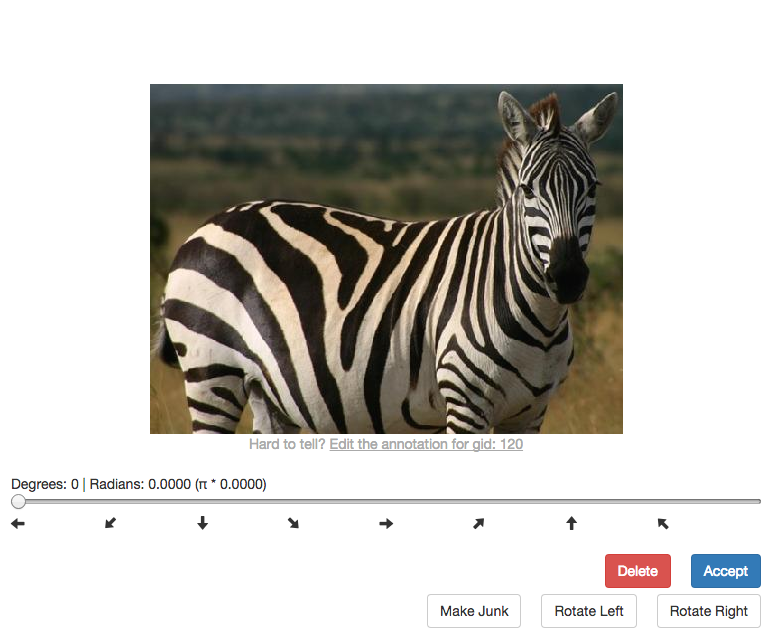
\includegraphics[width=0.75\textwidth]{resources/turk_viewpoint.png} }}$ }}%
        \caption[The Viewpoint Turking Web Interface]{\textbf{The Viewpoint Turking Web Interface.}  The viewpoint web interface allowed a reviewer to specify the viewpoint of the sighted animal.  The reviewer was given a bounding box annotation that was generated previously by the detection web interface.  The interface presented a slider signifying the viewpoint degree of the animal.  For example, the animal above would be given a viewpoint somewhere between \textit{front-right} ($4^{th}$ from the left) and \textit{right} ($5^{th}$ from the left), inclusive.  The interface also allowed for bounding box rotation (90 degrees left or right), editing, deletion, and a convenience button to mark the quality of the annotation as \textit{junk}.}
        \label{fig:turking_interface_viewpoint}
\end{figure}

The viewpoint of an animal was also useful information for building a robust image recognition database.  As more images are added to the database for a particular individual, there builds a degree of diminishing returns in terms of recognizability.  Furthermore, adding too many pictures of an individual can cause unnecessary imbalance to the search structure and can thus lead to poor recognition results.  With viewpoint annotation added to the individual's images, the identification algorithm pruned semantically duplicate images from the search structure, freeing up representational power for other individuals.  In practice, IBEIS typically limited the number of images to 2 for each of the eight viewpoints, for a maximum total of 16 images for an individual.

\begin{figure}[t]%
%\begin{figure}[!htb]%
    \centering
    \subfloat {{ $\vcenter{\hbox{ 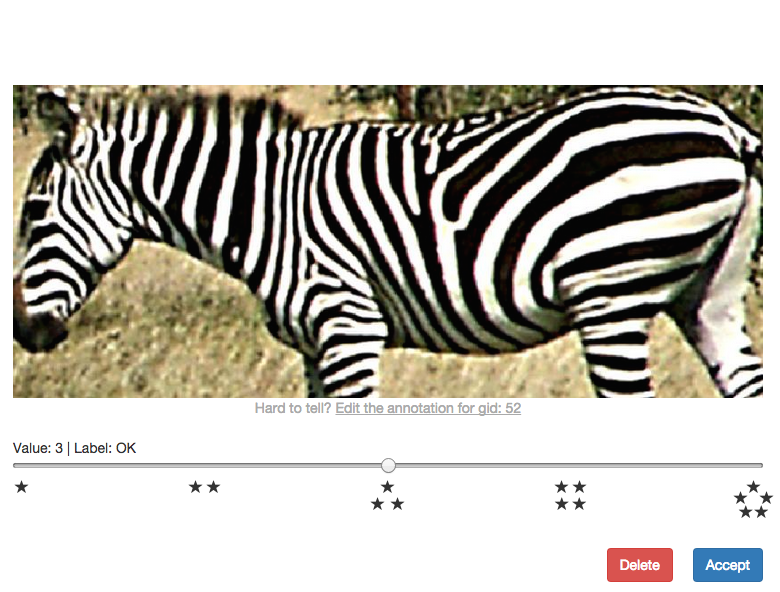
\includegraphics[width=0.75\textwidth]{resources/turk_quality.png} }}$ }}%
        \caption[The Quality Turking Web Interface]{\textbf{The Quality Turking Web Interface.}  The quality web interface allowed a reviewer to specify the quality of the sighting.  Again, the reviewer was given a bounding box annotation that was generated by the detection web interface.  The interface presented a 5-choice slider meant to signify the quality.  The above annotation is not blurred, has no obstructions, the animal is not occluded, and has good lighting.  However, the pixelization of the image degrades it to a 4-star (\textit{good}) quality.  The interface also allowed the reviewer to edit or delete the annotation.}
        \label{fig:turking_interface_quality}
\end{figure}

%\begin{figure*}[t]%
\begin{figure}[!htb]%
    \centering
    \subfloat[junk]{{ $\vcenter{\hbox{ 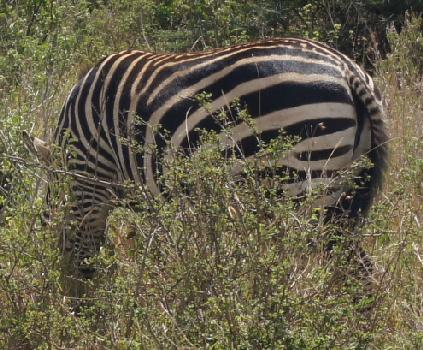
\includegraphics[width=0.22\textwidth]{resources/quality/quality-junk1.jpeg} }}$ }}%
    \subfloat[junk]{{ $\vcenter{\hbox{ 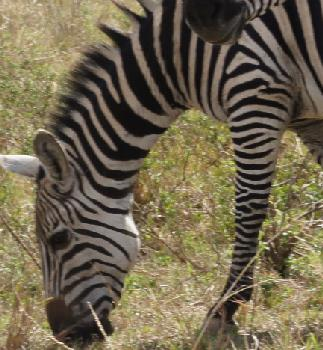
\includegraphics[width=0.22\textwidth]{resources/quality/quality-junk2.jpeg} }}$ }}%
    \subfloat[junk]{{ $\vcenter{\hbox{ 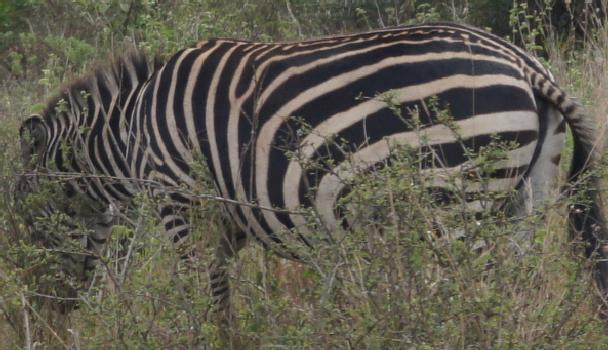
\includegraphics[width=0.22\textwidth]{resources/quality/quality-junk3.jpeg} }}$ }}%
    \vspace{0.1cm}
    \subfloat[poor]{{ $\vcenter{\hbox{ 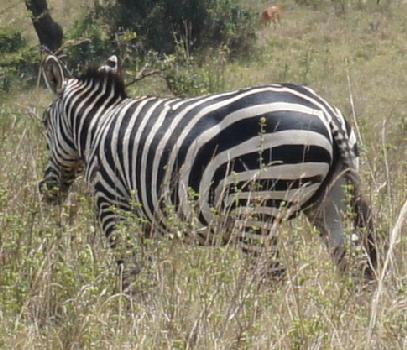
\includegraphics[width=0.22\textwidth]{resources/quality/quality-poor1.jpeg} }}$ }}%
    \subfloat[poor]{{ $\vcenter{\hbox{ 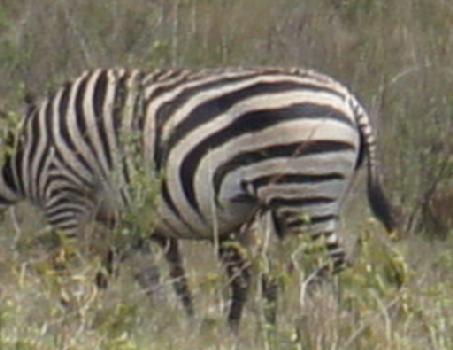
\includegraphics[width=0.22\textwidth]{resources/quality/quality-poor2.jpeg} }}$ }}%
    \subfloat[poor]{{ $\vcenter{\hbox{ 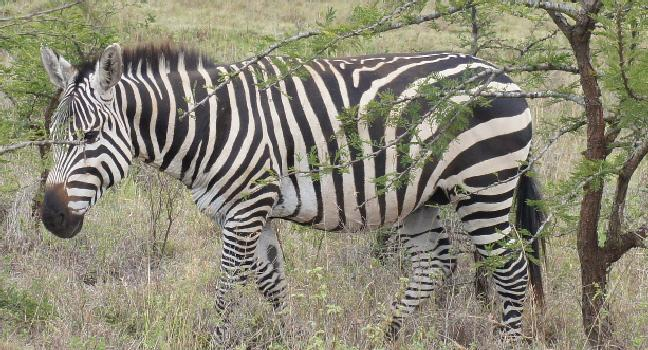
\includegraphics[width=0.22\textwidth]{resources/quality/quality-poor3.jpeg} }}$ }}%
    \vspace{0.1cm}
    \hrule
    \vspace{0.1cm}
    \subfloat[ok]{{ $\vcenter{\hbox{ 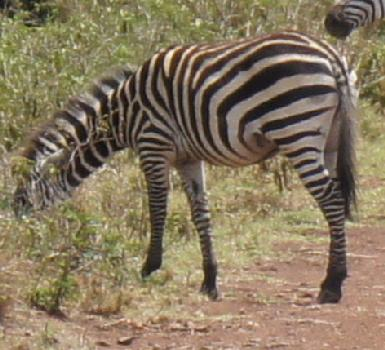
\includegraphics[width=0.22\textwidth]{resources/quality/quality-ok.jpeg} }}$ }}%
    \subfloat[good]{{ $\vcenter{\hbox{ 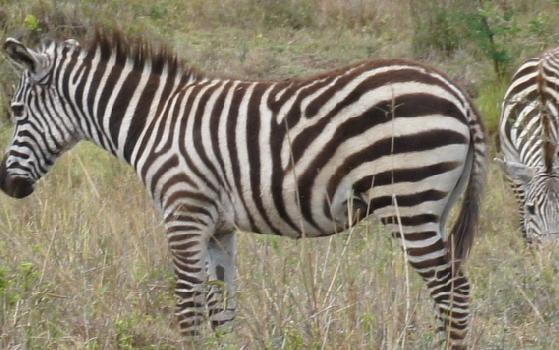
\includegraphics[width=0.22\textwidth]{resources/quality/quality-good.jpeg} }}$ }}%
    \subfloat[excellent]{{ $\vcenter{\hbox{ 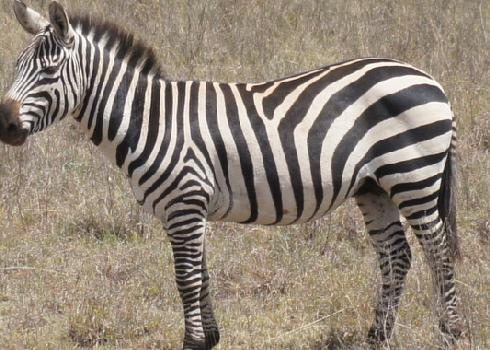
\includegraphics[width=0.22\textwidth]{resources/quality/quality-excellent.jpeg} }}$ }}%
    \vspace{0.1cm}
    \caption[Example Assigned Quality Scores for Images of Zebras]{\textbf{Example Assigned Quality Scores for Images of Zebras.}  The assigned quality scores for 9 images of zebras.  The \textit{junk} images (top row) have either extreme occlusion due to brush or due to only a small portion of the animal being photographed.  The \textit{poor} images (middle row), while also having occlusion issues, offer at least some usable information for identification, unlike the \textit{junk} images.  The final three quality metrics (bottom row) are assigned based on various levels of ideal pose, lighting conditions, and clarity.}
        \label{fig:qualities}
\end{figure}

Similar to viewpoint, an image was annotated with a quality score.  The quality score was designed to eliminate images that were blurry, poorly illuminated, the animal being too occluded by natural landscape or other animals, the animal being cut off for not being captured completely in the image, etc.  Ultimately, the quality score was also used to filter out images, that would have likely been noisy or otherwise poor for identification because the description extracted on these degraded images would have also been poor.  We wanted to maximize the chance of identifying an individual by only putting quality descriptors into the database, which only came from quality images.  An image was assigned a quality score of 1-5 stars -- \textit{junk}, \textit{poor}, \textit{ok}, \textit{good}, and \textit{excellent}, respectively -- with 1 being the lowest quality and 5 being the highest quality.  Examples of images with their assigned qualities can be seen in Figure \ref{fig:qualities}.  Looking at the figure, it is not easy to cleanly separate the examples for each quality score as it was largely subjective between reviewers.  Nevertheless, the quality was a consistent enough metric to discard poor images for processing.  For the GZGC, we processed all images that scored a quality of 3 (\textit{ok}) or higher.  During viewpoint annotation, the reviewer had the option of setting an image as being marked as \textit{junk}, as a convenience.  During quality annotation, the reviewer had the option of deleting the detection altogether.  An example image being reviewed in the web interface to be given a quality can be seen in Figure \ref{fig:turking_interface_quality}.

The quality metadata was also used to select the best images for an individual to be used in the recognition search structure.  As a result, viewpoint and quality share a similar utility of providing some form of cleanliness to the database.  %  It should be noted that no images of an individual were completely discarded, but instead were selectively included or ignored during the search database construction

\section{Identification} \label{sec:identification}
The IBEIS prototype for identifying animals was used during the GZGC analysis.  It is not a product of the current research of the author.  The identification algorithms, interfaces for identification and name conflict resolution, and computer vision techniques described in this section were developed by Jon Crall.  This section summarizes the IBEIS identification procedure.  Future Ph.D.\ dissertations will expand on the technical and algorithmic details of the software that powered the identification analysis.

Using viewpoint and quality as a filter, the detected image regions were passed into the IBEIS identification pipeline.  The images were compared to a database of individuals and the top ranking matches were returned for review.  A reviewer had the opportunity to select none, one, some, or all of the top matches in order to assign names and resolve naming conflicts.  An animal was then either assigned a new name and recorded in the database or assigned an existing name and its metadata was associated with that individual's sighting.

As a secondary identification procedure, we performed identification on the database against itself to identify mistakes made during naming.  The two scenarios are a name \textit{merge} and a name \textit{split}.  Name merges appeared as a single individual in the database under two (or more) different names.  The resolution for merged names was done as new sightings of individuals were added to the database.  Merging names was an integral part of the workflow as new sightings could offer new evidence or viewpoints that make merging the two names definitive.  However, not being careful in merging names for sightings lead to having to perform splits, a more demanding process.

A name split was needed when two or more individuals are in the database under the same name.  Name splits were difficult to identify in the database as the computational requirement to perform a comprehensive check was expensive.  In practice, name splits were detected by finding animals with an above-average number of sightings.  A name with a high number of sightings suggested that multiple animals were erroneously assigned to the same name.  For these animals, visual spot checking was sufficient to verify inconsistencies.  Once an inconsistency was identified, the assigned names were simply dropped for all sightings and identification for those images was redone.

\begin{figure}[t]%
%\begin{figure}[!htb]%
    \centering
    \subfloat {{ $\vcenter{\hbox{ 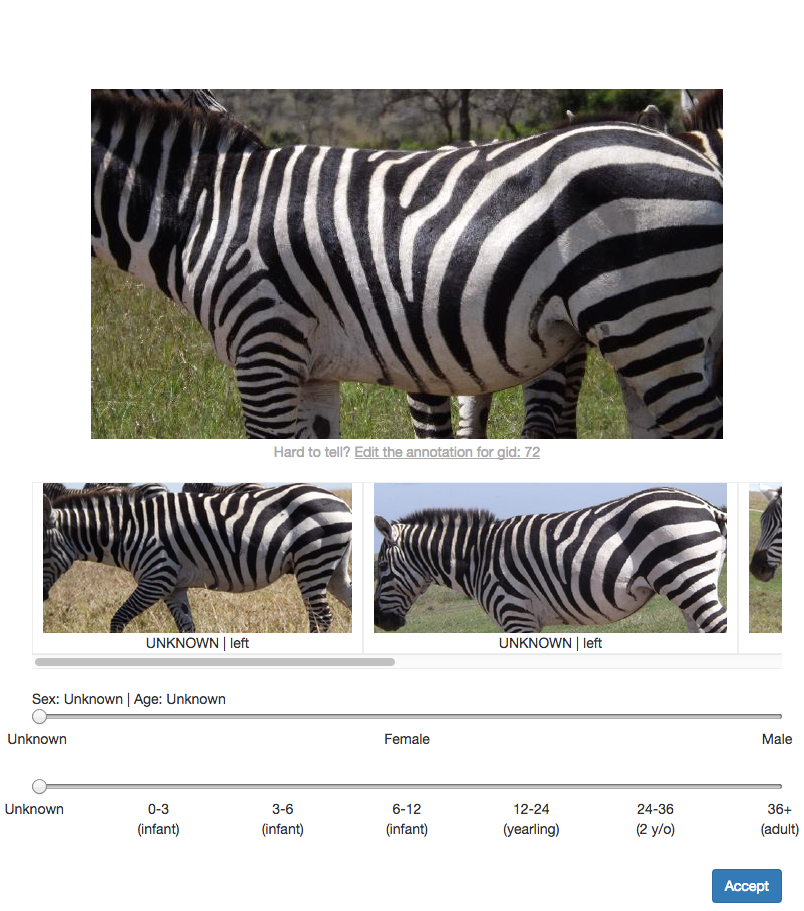
\includegraphics[width=0.75\textwidth]{resources/turk_metadata.png} }}$ }}%
        \caption[The Age and Sex Turking Web Interface]{\textbf{The Age and Sex Turking Web Interface.}  The age and sex web interface allowed a reviewer to (potentially) assign a sex and/or age to an animal.  This interface was meant to be used after names had been assigned by IBEIS.  As a result, multiple images of a named individual could be offered to help improve the accuracy.  The interface allowed for binned age groups and a gender determination through, again, the use of sliders.  Additional sightings of the same named individual were shown in a horizontal slider.  The reviewer could hover over one of the additional images to make it temporarily appear in the larger display above.}
        \label{fig:turking_interface_metadata}
\end{figure}

\section{Age and Sex}
To be able to analyze population demographics, we provided an interface for a reviewer to annotate the age and sex (when possible) for individuals.  The interface for adding age and sex was more or less the same as viewpoint and quality, but had the advantage of giving the reviewer multiple images of the same \textit{named individual} instead of a single image from a single sighting of an individual.  The advantage of being able to view multiple images of the same individual made the challenge of sexing the individual easier because multiple instances could be used to cross-reference for anatomical or behavioral traits of each sex.  Each individual zebra was given a sex of \textit{female}, \textit{male}, or \textit{unknown} and an age (in months) of 0-3 (\textit{infant}), 3-6 (\textit{infant}), 6-12 (\textit{infant}), 12-24 (\textit{yearling}), 24-36 (\textit{2-year-old}), or 36+ (\textit{adult}).  Figure
\ref{fig:turking_interface_metadata} shows the turking interface for aging and sexing an individual.

For the GZGC, we were able assign an age to the individuals because all images were collected over a period of only two weeks.  While sexing will always be done for an individual (applied to all images), the aging procedure would eventually have to be done on sightings only (each image at a time).  As the database matures over time, the age of an identified animal can be automatically inferred and the average life-expectancy for the zebra population can be estimated.

In summary, having web-accessible interfaces made the analysis of the data go much faster across all turking tasks.  The natural parallelization of web-based interfaces allowed for a seamless distribution to multiple concurrent reviewers and made analysis highly efficient.  All of the web interfaces shared a common visual design, which made it easier to train reviewers and allowed for smoother transitions between turking tasks.  The interfaces also utilized keyboard hotkey shortcuts (e.g.\ a number key to annotate quality, escape key to delete an annotation, etc.) for quickly annotating information.
